\subsection{Táblázatok}

%_
\begin{frame}
  \begin{columns}[c]
    \column{0.5\textwidth}
      Táblázatok alapértelmezett formázása:
      \begin{itemize}
        \item Cellaméretek a tartalomhoz igazodnak
        \item Nincsenek szegélyek
        \item Fejléc (\texttt{<th>}) cellák félkövérek, középre zártak
        \item Normál cellák (\texttt{<td>}) balra zártak
      \end{itemize}
    \column{0.45\textwidth}
        \begin{exampleblock}{\textattachfile{tablazat01.html}{tablazat01.html}}
          \begin{center}
            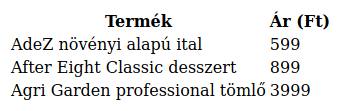
\includegraphics[width=\textwidth]{tablazat01.png}
          \end{center}
        \end{exampleblock}
  \end{columns}
\end{frame}

%_
\begin{frame}
  Kaphat szegélyt a teljes táblázat \dots
  \begin{columns}[c]
    \column{0.66\textwidth}
      \begin{exampleblock}{\textattachfile{tablazat02.html}{tablazat02.html}}
        \scriptsize
        \lstinputlisting[style=HTML,linerange={7-7},numbers=left,firstnumber=7]{tablazat02.html}
        \lstinputlisting[style=HTML,linerange={11-16},numbers=left,firstnumber=11]{tablazat02.html}
      \end{exampleblock}
    \column{0.3\textwidth}
      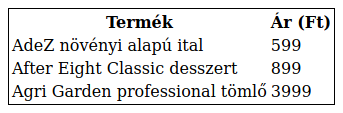
\includegraphics[width=\textwidth]{tablazat02.png}
  \end{columns}
\end{frame}

%_
\begin{frame}
  \dots vagy annak cellái \dots
  \vfill
  \begin{exampleblock}{\textattachfile{tablazat03.html}{tablazat03.html}}
    \lstinputlisting[style=HTML,linerange={7-7},numbers=left,firstnumber=7]{tablazat03.html}
  \end{exampleblock}
  \begin{center}
    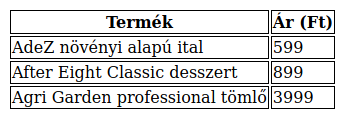
\includegraphics[width=0.4\textwidth]{tablazat03.png}
  \end{center}
\end{frame}

%_
\begin{frame}
  \dots vagy mindkettő.
  \vfill
  \begin{exampleblock}{\textattachfile{tablazat04.html}{tablazat04.html}}
    \lstinputlisting[style=HTML,linerange={7-7},numbers=left,firstnumber=7]{tablazat04.html}
  \end{exampleblock}
  \begin{center}
    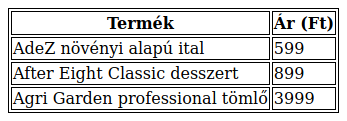
\includegraphics[width=0.4\textwidth]{tablazat04.png}
  \end{center}
\end{frame}

%_
\begin{frame}
  A cellák közötti távolság változtatható a \texttt{<table>} \texttt{border-spacing} tulajdonságával \dots
  \vfill
  \begin{exampleblock}{\textattachfile{tablazat05.html}{tablazat05.html}}
    \lstinputlisting[style=HTML,linerange={7-8},numbers=left,firstnumber=7]{tablazat05.html}
  \end{exampleblock}
  \begin{center}
    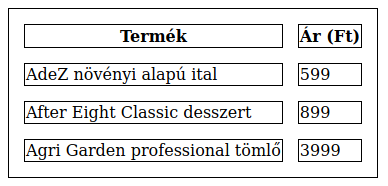
\includegraphics[width=0.4\textwidth]{tablazat05.png}
  \end{center}
\end{frame}

%_
\begin{frame}
  \dots de teljesen el is tüntethető a \texttt{<table>} \texttt{border-collapse} tulajdonságával:
  \begin{description}[m]
    \item[\texttt{separate}] elkülönített cellák, alapértelmezés.
    \item[\texttt{collapse}] összevont cellaszegélyek.
  \end{description}
  \vfill
  \begin{exampleblock}{\textattachfile{tablazat06.html}{tablazat06.html}}
    \lstinputlisting[style=HTML,linerange={7-8},numbers=left,firstnumber=7]{tablazat06.html}
  \end{exampleblock}
  \begin{center}
    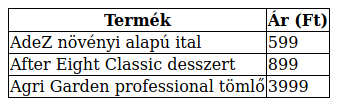
\includegraphics[width=0.4\textwidth]{tablazat06.png}
  \end{center}
\end{frame}

%_
\begin{frame}
  A cellák szegélye és tartalma közötti távolság a \texttt{<td>}, \texttt{<th>} \texttt{padding} tulajdonságával állítható.
  \begin{exampleblock}{\textattachfile{tablazat07.html}{tablazat07.html}}
    \footnotesize
    \lstinputlisting[style=HTML,linerange={7-11},numbers=left,firstnumber=7]{tablazat07.html}
  \end{exampleblock}
  \begin{center}
    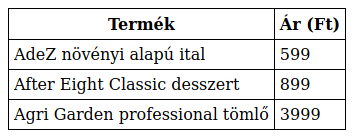
\includegraphics[width=0.4\textwidth]{tablazat07.png}
  \end{center}
\end{frame}

%_
\begin{frame}
  A cellákon belüli igazítás a \texttt{text-align}, \texttt{vertical-align} tulajdonságokkal állítható.
  \begin{exampleblock}{\textattachfile{tablazat08.html}{tablazat08.html}}
    \scriptsize
    \lstinputlisting[style=HTML,linerange={7-13},numbers=left,firstnumber=7]{tablazat08.html}
  \end{exampleblock}
  \begin{center}
    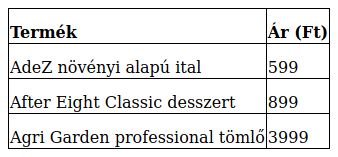
\includegraphics[width=0.35\textwidth]{tablazat08.png}
  \end{center}
\end{frame}

%_
\begin{frame}
  Ha a táblázat szélesebb, mint amit a tartalom indokol, a maradék hely arányosan lesz elosztva.
  \begin{exampleblock}{\textattachfile{tablazat09.html}{tablazat09.html}}
    \scriptsize
    \lstinputlisting[style=HTML,linerange={7-14},numbers=left,firstnumber=7]{tablazat09.html}
  \end{exampleblock}
  \begin{center}
    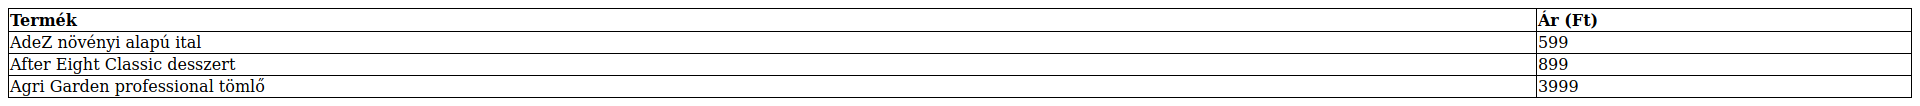
\includegraphics[width=\textwidth]{tablazat09.png}
  \end{center}
\end{frame}

%_
\begin{frame}
  \begin{columns}[c]
    \column{0.3\textwidth}
      \small
      Az olvashatóság javításához pl. kiemelhetjük az egér alatti sort a \texttt{:hover} látszólagos osztállyal.\\
      Figyeljük meg a ,,csíkozást''!
      \vfill
      \begin{center}
        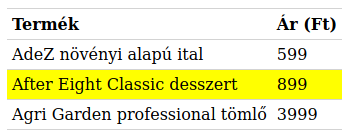
\includegraphics[width=\textwidth]{tablazat10.png}
      \end{center}
    \column{0.66\textwidth}
      \begin{exampleblock}{\textattachfile{tablazat10.html}{tablazat10.html}}
        \scriptsize
        \lstinputlisting[style=HTML,linerange={7-16},numbers=right,firstnumber=7]{tablazat10.html}
      \end{exampleblock}
  \end{columns}
\end{frame}

%_
\begin{frame}
  Az olvashatóság a sorok váltakozó háttérszínével is javítható. Egy szülő elem (pl. \texttt{<table>}) gyerekei (sorok) közül meghatározottak kiválasztása: \hiv{\href{https://developer.mozilla.org/en-US/docs/Web/CSS/:nth-child}{\texttt{nth-child()}}} látszólagos osztállyal.
  \begin{columns}[c]
    \column{0.66\textwidth}
      \begin{description}[m]
        \item[\texttt{An+b}] \hfill \\ $n = 0 \dots$, de a gyerekek számozása 1-től indul!
        \item[\texttt{even}] \hfill \\ Páros elemek $\equiv$ \texttt{2n}
        \item[\texttt{odd}] \hfill \\ Páratlan elemek $\equiv$ \texttt{2n+1}
      \end{description}
    \column{0.3\textwidth}
      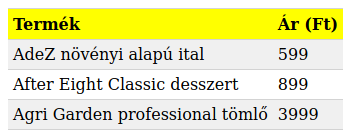
\includegraphics[width=\textwidth]{tablazat11.png}
  \end{columns} 
\end{frame}

%_
\begin{frame}
  \begin{exampleblock}{\textattachfile{tablazat11.html}{tablazat11.html}}
    \small
    \lstinputlisting[style=HTML,linerange={7-17},numbers=left,firstnumber=7]{tablazat11.html}
  \end{exampleblock}
\end{frame}

%_
\begin{frame}
  \begin{columns}[c]
    \column{0.66\textwidth}
      Görgethető táblázat, trükkök:
      \begin{itemize}
        \item Rögzített fejléc $\to$ két külön táblázat, csak az alsó görgethető
        \item Görgetés: táblázat beágyazva egy túl alacsony elembe, és \texttt{overflow-y: scroll} (hasonlóan a vízszintes irányú görgetés is lehetséges az \texttt{overflow-x} tulajdonsággal)
        \item Legyenek a két táblázat oszlopai rendre azonos szélességűek!
      \end{itemize}
    \column{0.3\textwidth}
      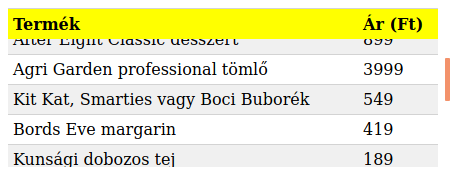
\includegraphics[width=\textwidth]{tablazat12.png}
  \end{columns}
\end{frame}

%_
\begin{frame}
  \begin{exampleblock}{\textattachfile{tablazat12.html}{tablazat12.html}}
    \fontsize{7}{8} \selectfont
    \lstinputlisting[style=HTML,linerange={28-41},numbers=left,firstnumber=28]{tablazat12.html}
    \lstinputlisting[style=HTML,linerange={51-53},numbers=left,firstnumber=51]{tablazat12.html}
  \end{exampleblock}
\end{frame}

%_
\begin{frame}
  \begin{exampleblock}{\textattachfile{tablazat12.html}{tablazat12.html}}
    \fontsize{7}{8} \selectfont
    \lstinputlisting[style=HTML,linerange={7-24},numbers=left,firstnumber=7]{tablazat12.html}
  \end{exampleblock}
\end{frame}

%_
\begin{frame}
  Táblázat címkéjének elhelyezése: \texttt{caption-side}
  \begin{description}[m]
    \item[\texttt{top}] \hfill \\ Fent, alapértelmezés.
    \item[\texttt{bottom}] \hfill \\ Lent.
  \end{description}
  \vfill
  Üres cellák szegélyeinek rajzolása: \texttt{empty-cells}
  \begin{description}[m]
    \item[\texttt{show}] \hfill \\ Megrajzolja, alapértelmezés.
    \item[\texttt{hide}] \hfill \\ Nem rajzolja meg.
  \end{description}
\end{frame}

%_
\begin{frame}
  Táblázat megjelenítési algoritmus: \texttt{table-layout}
  \begin{description}[m]
    \item[\texttt{auto}] \hfill \\ A cellák szélessége a legszélesebb nem tördelhető tartalmi elem függvénye. Alapértelmezés.
    \item[\texttt{fixed}] \hfill \\ Az oszlopok szélességét vagy
    \begin{itemize}
      \item a \texttt{<table>} és \texttt{<col>} elemek szélességei adják meg, vagy
      \item az első sor celláinak szélességei. Ha ilyen nincs, egyforma szélesek lesznek a cellák.
    \end{itemize}
    Nagy táblázatoknál jelentősen gyorsabb megjelenés.
  \end{description}
\end{frame}

%_
\begin{frame}
  Készítse el a \textattachfile{queen.png}{queen.png} fájl felhasználásával az alábbi weboldalt, ami a \hiv{\href{https://hu.wikipedia.org/wiki/Nyolckir\%C3\%A1lyn\%C5\%91-probl\%C3\%A9ma}{Nyolckirálynő probléma}} egy lehetséges megoldását mutatja! Ügyeljen rá, hogy keskeny kijelzőkön a táblázat vízszintesen görgethető legyen! (A cellák 50x50, a képek 40x40px méretűek.)
  \begin{exampleblock}{\textattachfile{sakk.html}{sakk.html}}
    \begin{center}
      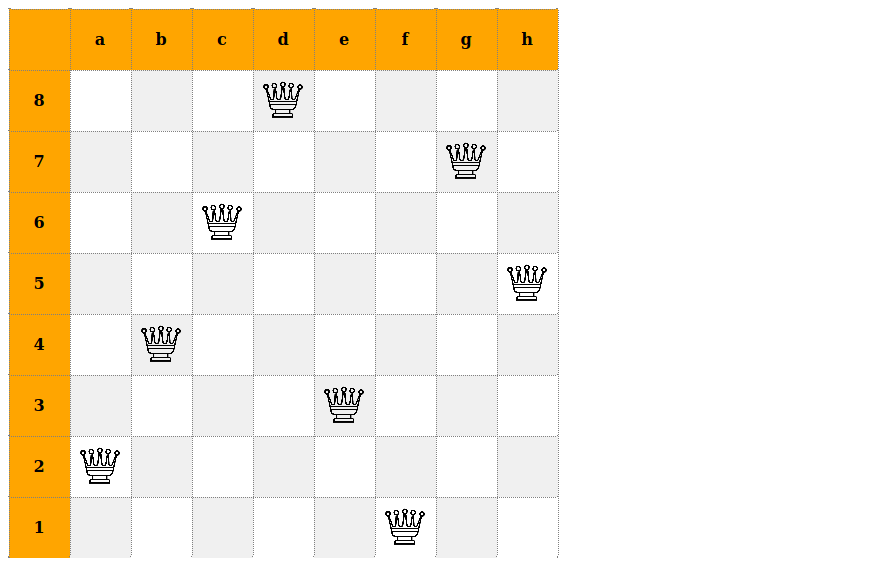
\includegraphics[scale=0.15]{sakk1.png}\hspace{1cm}
      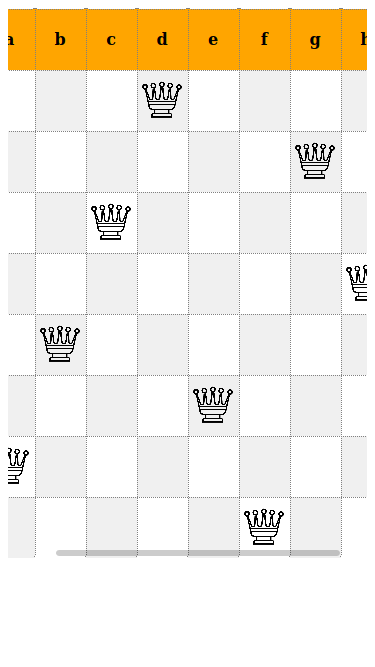
\includegraphics[scale=0.15]{sakk2.png}
    \end{center}
  \end{exampleblock}  
\end{frame}
